\documentclass[11pt,letterpaper,twocolumn]{article}

\usepackage[utf8]{inputenc}
\usepackage[portuguese]{babel}
\usepackage{float}
\usepackage{xcolor}
\usepackage{verbatim}
\usepackage{charter}
\usepackage{amsmath}
\usepackage{appendix}
\usepackage{ragged2e}
\usepackage{array}
\usepackage{etoolbox}
\usepackage{fancyhdr}
\usepackage{booktabs}
\usepackage{arydshln}
\usepackage{caption}
\usepackage{subcaption}
\usepackage{enumitem}
\usepackage[bottom=3 cm,top=2.0cm,left=2.0cm,right=2.0cm]{geometry}
\usepackage{graphicx}
\usepackage{mathtools}
\usepackage{multirow}
\usepackage{pdfpages}
\usepackage{subfiles}
\usepackage[compact]{titlesec}
\usepackage{stfloats}
\usepackage{hyperref}
\usepackage{amsfonts}
\usepackage[export]{adjustbox}


\setlength{\columnsep}{30pt}

%\titlelabel{\thetitle.\quad}

\pagestyle{fancy}
\fancyhf{}
      
\fancyfoot{}
\fancyfoot[C]{\thepage} % page
\renewcommand{\headrulewidth}{0mm} % headrule width
\renewcommand{\footrulewidth}{0mm} % footrule width

\makeatletter
\patchcmd{\headrule}{\hrule}{\color{black}\hrule}{}{} % headrule
\patchcmd{\footrule}{\hrule}{\color{black}\hrule}{}{} % footrule
\makeatother

\definecolor{blueM}{cmyk}{1.0,0.49,0.0,0.47}
    
\begin{document}
\twocolumn[\begin{@twocolumnfalse}

\begin{minipage}{\textwidth}
\vspace{5mm}
    \Large{\textbf{Inferência Causal sobre a renda anual da população norte-americana}} 
    \vspace{3mm}
    
    \large{\textbf{Igor Patrício Michels}} 
    \vspace{2mm}\newline

    \fontsize{0.35cm}{0.5cm}\selectfont \textit{Escola de Matemática Aplicada, EMAp/FGV\newline 
    Rio de Janeiro/RJ, Brasil}
    \vspace{1mm} 
    
    \today

\end{minipage}

\small
\vspace{11pt}
\centerline{\rule{0.95\textwidth}{0.4pt}}

\begin{center}
    \begin{minipage}{0.9\textwidth}
        \noindent \textbf{Resumo:}
        Esse trabalho tem como objetivo analisar quais características detém maior relevância na tentativa de predizer o salário de um determinado indivíduo. A análise se dará por meio de DAGs - Directed Acyclic Graphs - em ambiente computacional.
        \vspace{4mm}
        
        \noindent \textbf{Palavras chave:} DAGs, Inferência Causal, Análise de Renda.
    \end{minipage}
\end{center}

\centerline{\rule{0.95\textwidth}{0.4pt}}

\vspace{15pt}
\end{@twocolumnfalse}]

\section{Introdução}
\justify

Em diversas situações do cotidiano a renda de um indivíduo é relevante. Seja para a realização de um empréstimo bancário, seja na realização de um financiamento ou para o pleito de algum benefício social como, por exemplo, bolsas de estudos. Nesse sentido, muitas vezes é necessário uma maior comprovação de renda, bem como uma fiscalização para evitar, ao máximo, que hajam beneficiários sem os devidos direitos. Com isso, diversos estudos surgem com o intuito de modelar a renda de um indivíduo por meio de dados sociais do mesmo. Mas quais dados devem ser mais relevantes para tal modelagem?

Dessa forma, esse estudo surge pensando em modelar a estrutura causal de um modelo de renda de indivíduos por meio de DAGs - Directed Acyclic Graphs - além de apresentar a ideia do mesmo para a inferência causal.

\section{Metodologia}
\justify

Conforme citado anteriormente, o objetivo desse estudo é ilustrar o funcionamento da modelagem com DAGs por meio da realização de uma análise causal da renda anual de uma população de norte-americanos, analisando quais atributos mostram ter maior relevância para uma renda anual maior ou igual a de \$50.000,00. Para tanto, os dados cujas análises se referem foram encontrados em \cite{dua2019}. As análises foram realizadas em R com uma análise similar a encontrada em \cite{ct}.

A escolha pela linguagem R se deve pela facilidade da implementação de uma análise causal com DAGs por meio de ferramentas oriundas da biblioteca {\fontfamily{pcr}\selectfont Dagitty}.

\section{Directed Acyclic Graphs}

Primeiramente iremos abordar brevemente nosso objeto de estudo, ou seja, o DAG. Um DAG nada mais é que um grafo acíclico direcionado, isso é, para cada um dos vértices $v$ do grafo, não existe um caminho direcionado que parte de $v$ e chega a $v$. Por tal propriedade, o DAG é comumente usado para modelar fenômenos em que não faz sentido um objeto (uma classe, por exemplo) ter relação consiga mesmo.

No contexto da inferência causal, pode-se utilizar os DAGs como forma de representar a estrutura em estudo. Essa possibilidade se dá pela existência de um ordenamento topológico em um DAG, isso é, quando trabalha-se com um DAG sempre existe um ordenamento dos vértices de modo que as ligações apontam sempre para o mesmo sentido. Visualmente, pode-se interpretar que, ao enfileirar todos os vértices em uma mesma linha horizontal, sempre existe alguma permutação dos vértices de modo que as arestas sempre partem de um vértice da esquerda para algum da direita. Um exemplo de ordenamento topológico pode ser visto na Figura \ref{ord_top}.
\begin{figure}
    \centering
    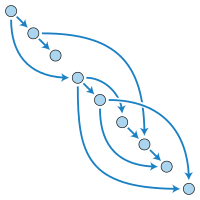
\includegraphics{A2/Imagens/Topological_Ordering.png}
    \caption{Ordenamento topológico de um grafo. Note que toda aresta do grafo saí de um vértice que está acima e à esquerda do vértice para o qual a mesma está apontando.}
    \label{ord_top}
\end{figure}

Essa representação, e consequentemente, a estrutura de um DAG, permite interpretar o mesmo como um diagrama causal, isso é, se um vértice $A$ contém uma aresta que está apontando para o vértice $B$, então pode-se interpretar $B$ como uma causa de $A$, o que vai permitir a realização de análises causais.

\section{Modelagem}
\justify

Conforme citado anteriormente, os dados foram extraídos de \cite{dua2019}, de um banco de dados para previsão de renda anual, isso é, se um indivíduo recebe ou não mais que \$50.000,00 anuais. Entretanto, como o objetivo desse trabalho é um pouco diferente, acabou se utilizando apenas o dataset de treino para realizar a modelagem, o qual, após limpar os dados, contava com dados de aproximadamente 30000 indivíduos. Na Figura \ref{table1} pode-se ver o dataset antes da limpeza, enquanto a Figura \ref{table2} apresenta o mesmo após a limpeza e alteração dos dados.
\begin{figure}
    \centering
    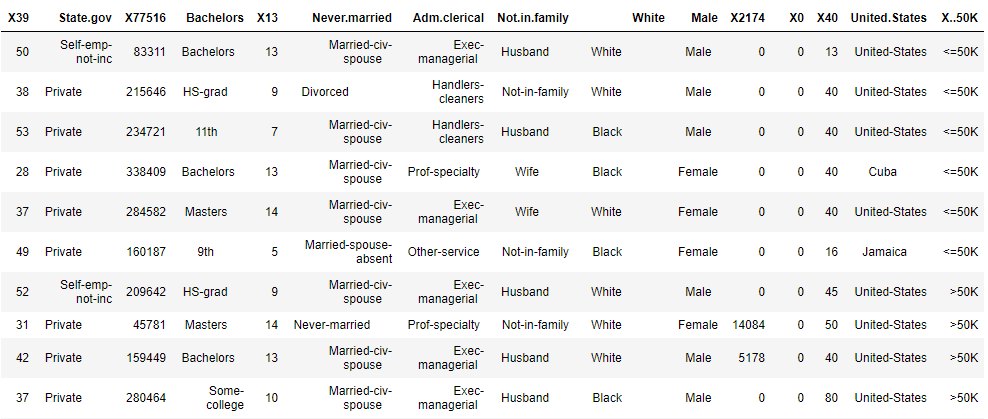
\includegraphics[scale = 0.3]{A2/Imagens/table1.png}
    \caption{Dados antes da limpeza}
    \label{table1}
\end{figure}

\begin{figure}
    \centering
    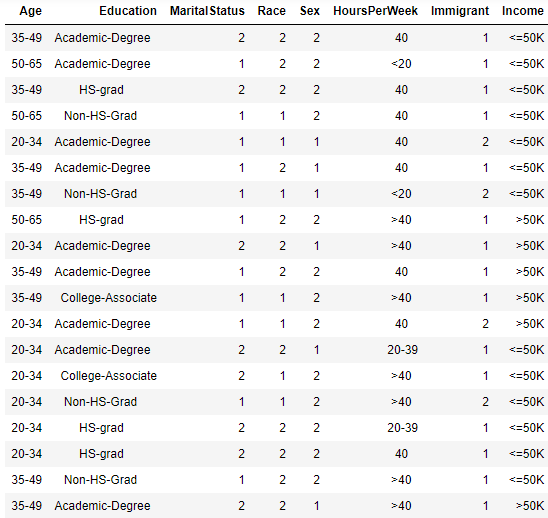
\includegraphics[scale = 0.5]{A2/Imagens/table2.png}
    \caption{Dados após a limpeza}
    \label{table2}
\end{figure}

Na limpeza foram criados alguns ``grupos'' de indivíduos, seja pela idade, grau de instrução, etc. Note que algumas características que eram multi-categóricas viraram binárias (possuindo valores $1$ ou $2$), isso se dá pela falta de um ordenamento natural dos dados, isso é, a variável que representa grau de instrução continuou com várias categorias por que as mesmas são ordenáveis: Non-HS-Grad, HS-grad, College-Associate e, por fim, Academic-Degree. Já categorias como o estado civil não tem um ordenamento natural, isso é, ser solteiro não necessariamente vem antes de ser casado, pois você pode se casar e depois se divorciar, voltando a estar solteiro. Dessa forma, optou-se pela variável binária onde $1$ representa que o indivíduo é casado e $2$ significa que ele não é casado (pode ser solteiro, divorciado, viúvo, etc). Por fim, as variáveis ``Race'', ``Sex'' e ``Imigrant'' seguem a mesma lógica, onde ``Race'' sendo $2$ significa que a pessoa é branca e $1$ significa que não é, para ``Sex'', $2$ representa os homens e $1$ as mulheres, enquanto que para ``Imigrant'' $1$ representa que não é imigrante, ou seja, um estadunidense, enquanto que $2$ representa que é imigrante.

Feito isso, pode-se partir para a modelagem das relações causais desse sistema. Um modelo pode ser visto na Figura \ref{model1}.
\begin{figure}
    \centering
    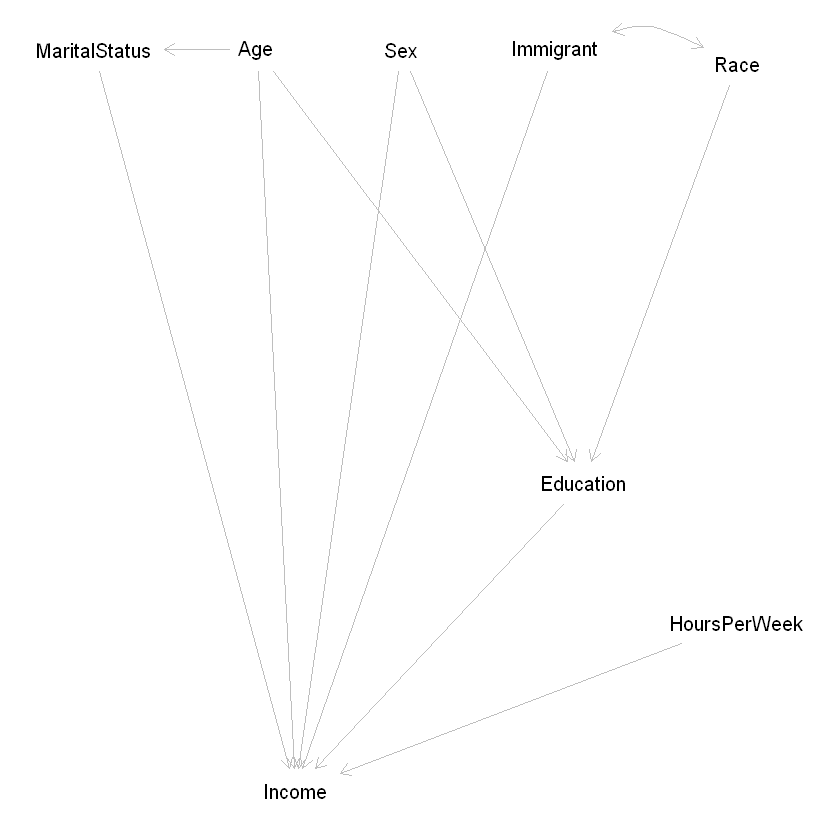
\includegraphics[scale = 0.5]{A2/Imagens/model1.png}
    \caption{Modelo causal proposto}
    \label{model1}
\end{figure}

As conexões da Figura \ref{model1} podem ser explicadas a partir do pensamento que pessoas casadas buscam uma maior renda, pois em geral as mesmas possuem mais despesas com o que se preocupar. O mesmo se aplica para a idade, a qual também ajuda a explicar a variável referente ao estado civil, pois não é esperado que um jovem de, por exemplo, 18 anos, seja casado. O sexo do indivíduo também ajuda a explicar a renda, uma vez que historicamente as mulheres são menos valorizadas, mesmo ocupando o mesmo cargo que um homem. Junto com a raça do indivíduo, o sexo e a idade acabam explicando a educação do mesmo, seja quanto a nível ou qualidade. O fator imigrante é considerado com a ideia de que muitos imigrantes acabam aceitando qualquer oferta de emprego ao chegar nos Estados Unidos de modo a não ficar à mercê da sorte. Já a relação entre raça e imigrantes se dá pela composição racial do país analisado, onde, em geral, os imigrantes tendem a fugir da mesma. Por fim, a carga horária semanal é considerada com o intuito de diferenciar empregos de baixa carga horária para empregos com alta carga horária, uma vez que o esperado é que a carga horária seja, de certa forma, proporcional ao salário de um indivíduo.

Um outro modelo explorado se dá pelos dados do sexo e imigrante atuando por meio da carga horária, com a idade também tendo influência sobre a mesma, conforme pode ser visto na Figura \ref{model2}.
\begin{figure}
    \centering
    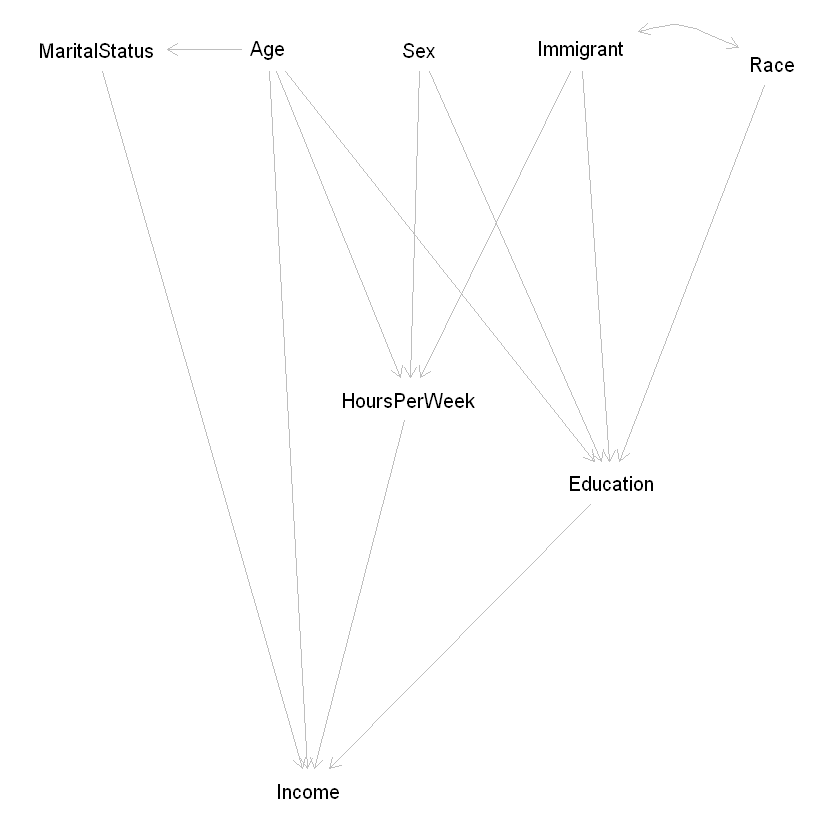
\includegraphics[scale = 0.5]{A2/Imagens/model2.png}
    \caption{Modelo causal proposto}
    \label{model2}
\end{figure}

\section{Resultados}
\justify

Primeiramente, irei abordar os resultados do modelo visto na Figura \ref{model1}. Para tanto, podemos analisar o comportamento das variáveis que o modelo trata como independentes. O resultado da análise pode ser visto na Tabela \ref{r1m1}, onde a estimativa é a da correlação entre as variáveis, o p-valor corresponde a hipótese de que as variáveis são independentes, ou seja, correlação nula, e as demais colunas apresentam os limites para um intervalo de confiança de 95\%.
\begin{table*}[ht]
    \centering
    \begin{tabular}{rrrrr}
        \hline
        & estimate & p.value & 2.5\% & 97.5\% \\ 
        \hline
        Age \_$||$\_ HrPW & 0.14 & 0.00 & 0.13 & 0.15 \\ 
        Age \_$||$\_ Immg & -0.01 & 0.02 & -0.03 & -0.00 \\ 
        Age \_$||$\_ Race & 0.02 & 0.00 & 0.01 & 0.03 \\ 
        Age \_$||$\_ Sex & 0.09 & 0.00 & 0.08 & 0.10 \\ 
        Edct \_$||$\_ HrPW & 0.20 & 0.00 & 0.19 & 0.21 \\ 
        Edct \_$||$\_ Immg $|$ Race & -0.08 & 0.00 & -0.09 & -0.07 \\ 
        Edct \_$||$\_ MrtS $|$ Age & -0.05 & 0.00 & -0.06 & -0.04 \\ 
        HrPW \_$||$\_ Immg & -0.03 & 0.00 & -0.04 & -0.02 \\ 
        HrPW \_$||$\_ MrtS & -0.26 & 0.00 & -0.27 & -0.25 \\ 
        HrPW \_$||$\_ Race & 0.09 & 0.00 & 0.08 & 0.10 \\ 
        HrPW \_$||$\_ Sex & 0.28 & 0.00 & 0.27 & 0.29 \\ 
        Immg \_$||$\_ MrtS & -0.03 & 0.00 & -0.04 & -0.02 \\ 
        Immg \_$||$\_ Sex & 0.00 & 0.60 & -0.01 & 0.01 \\ 
        Incm \_$||$\_ Race $|$ Age, Edct, Immg, Sex & 0.08 & 0.00 & 0.07 & 0.09 \\ 
        MrtS \_$||$\_ Race & -0.10 & 0.00 & -0.11 & -0.09 \\ 
        MrtS \_$||$\_ Sex & -0.43 & 0.00 & -0.44 & -0.42 \\ 
        Race \_$||$\_ Sex & 0.11 & 0.00 & 0.09 & 0.12 \\ 
        \hline
    \end{tabular}
    \caption{Resultados para o modelo da Figura \ref{model1}.}
    \label{r1m1}
\end{table*}

Idealmente, todos os valores estimados deveriam ficar próximos do zero. Visualmente, no cenário em que todas as variáveis são independentes, todos os pontos ficariam sobre a linha vertical na Figura \ref{r1m1f}.
\begin{figure}
    \centering
    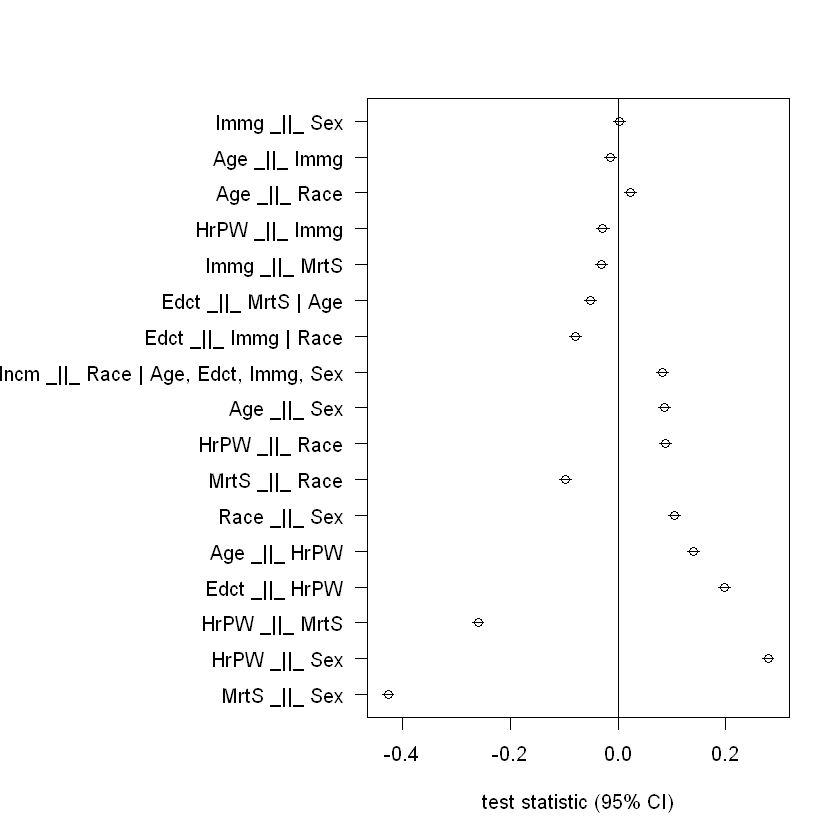
\includegraphics[scale = 0.5]{A2/Imagens/r1m1.png}
    \caption{Dados da Tabela \ref{r1m1} em uma representação visual.}
    \label{r1m1f}
\end{figure}

Note que alguns dados não demonstram ser independentes, como, por exemplo, o estado civil e o sexo. Esse exemplo, em particular, se dá pela natureza do dataset, o qual foi coletado em uma época em que o casamento nos EUA era apenas entre homens e mulheres, logo, em uma amostra da população, a proporção de homens casados deve ser similar a de mulheres casadas, mas isso não ocorre nesse dataset, onde temos uma proporção muito maior de homens casados em relação a mulheres, o que leva o modelo de encontro a essa correlação negativa. Uma outra correlação alta obtida com esse modelo é a do sexo com a carga horária semanal. Dessa forma, vemos que o primeiro modelo, apresentado na Figura \ref{model1} é ligeiramente menos eficaz que o segundo modelo, apresentado na Figura \ref{model2}, o qual já traz consigo a noção de causa e efeito entre o sexo do indivíduo e a carga horária semanal do mesmo.

Dito isso, podemos analisar os resultados do segundo modelo, apresentados na Tabela \ref{r1m2}.
\begin{table*}[ht]
    \centering
    \begin{tabular}{rrrrr}
        \hline
        & estimate & p.value & 2.5\% & 97.5\% \\ 
        \hline
        Age \_$||$\_ HrPW & 0.14 & 0.00 & 0.13 & 0.15 \\ 
        Age \_$||$\_ Immg & -0.01 & 0.02 & -0.03 & -0.00 \\ 
        Age \_$||$\_ Race & 0.02 & 0.00 & 0.01 & 0.03 \\ 
        Age \_$||$\_ Sex & 0.09 & 0.00 & 0.08 & 0.10 \\ 
        Edct \_$||$\_ HrPW & 0.20 & 0.00 & 0.19 & 0.21 \\ 
        Edct \_$||$\_ Immg $|$ Race & -0.08 & 0.00 & -0.09 & -0.07 \\ 
        Edct \_$||$\_ MrtS $|$ Age & -0.05 & 0.00 & -0.06 & -0.04 \\ 
        HrPW \_$||$\_ Immg & -0.03 & 0.00 & -0.04 & -0.02 \\ 
        HrPW \_$||$\_ MrtS & -0.26 & 0.00 & -0.27 & -0.25 \\ 
        HrPW \_$||$\_ Race & 0.09 & 0.00 & 0.08 & 0.10 \\ 
        HrPW \_$||$\_ Sex & 0.28 & 0.00 & 0.27 & 0.29 \\ 
        Immg \_$||$\_ MrtS & -0.03 & 0.00 & -0.04 & -0.02 \\ 
        Immg \_$||$\_ Sex & 0.00 & 0.60 & -0.01 & 0.01 \\ 
        MrtS \_$||$\_ Race & -0.10 & 0.00 & -0.11 & -0.09 \\ 
        MrtS \_$||$\_ Sex & -0.43 & 0.00 & -0.44 & -0.42 \\ 
        Race \_$||$\_ Sex & 0.11 & 0.00 & 0.09 & 0.12 \\ 
        \hline
    \end{tabular}
    \caption{Resultados para o modelo da Figura \ref{model2}.}
    \label{r1m2}
\end{table*}

De forma análoga aos resultados anteriores, podemos analisar esses resultados em um gráfico, conforme disposto na Figura \ref{r1m2f}.
\begin{figure}
    \centering
    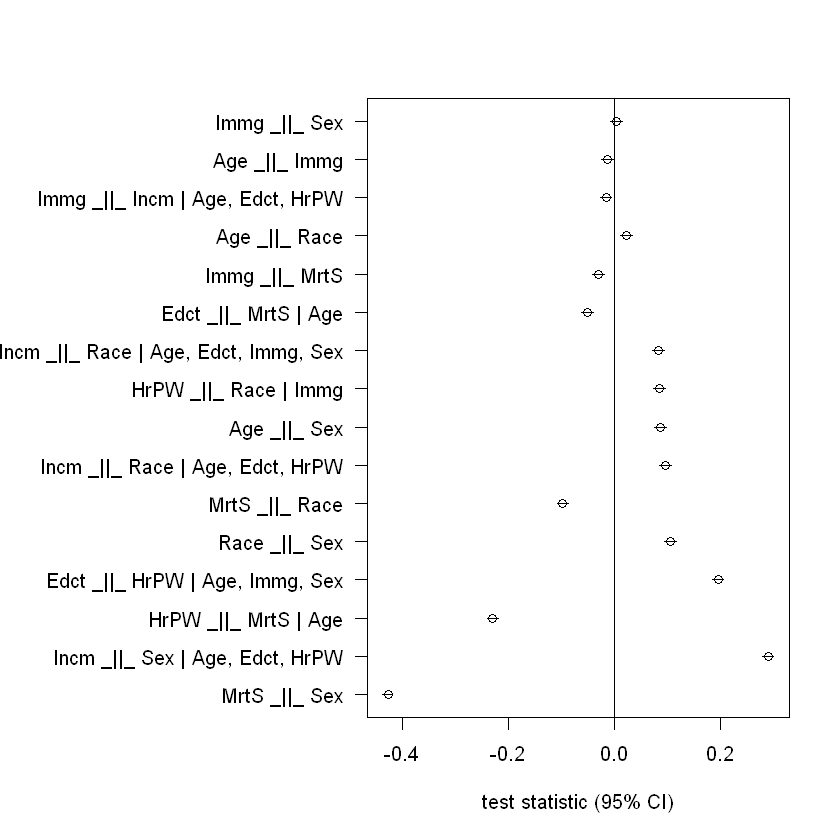
\includegraphics[scale = 0.5]{A2/Imagens/r1m2.png}
    \caption{Dados da Tabela \ref{r1m2} em uma representação visual.}
    \label{r1m2f}
\end{figure}

Note que a inclusão da dependência da carga horária semanal para o sexo, idade e variável binária imigrante geraram análises mais complexas, como a da correlação das variáveis Income com Race, por meio das variáveis Age, Education, Immigrant e Sex, o que pode acabar deixando a análise cada vez mais complexa. Dessa forma, podemos fazer a análise limitando a uma variável intermediadora, conforme pode ser observado na Tabela \ref{r2m2}.
\begin{table*}[ht]
    \centering
    \begin{tabular}{rrrrr}
        \hline
        & estimate & p.value & 2.5\% & 97.5\% \\ 
        \hline
        Age \_$||$\_ Immg & -0.01 & 0.02 & -0.03 & -0.00 \\ 
        Age \_$||$\_ Race & 0.02 & 0.00 & 0.01 & 0.03 \\ 
        Age \_$||$\_ Sex & 0.09 & 0.00 & 0.08 & 0.10 \\ 
        Edct \_$||$\_ MrtS $|$ Age & -0.05 & 0.00 & -0.06 & -0.04 \\ 
        HrPW \_$||$\_ MrtS $|$ Age & -0.23 & 0.00 & -0.24 & -0.22 \\ 
        HrPW \_$||$\_ Race $|$ Immg & 0.08 & 0.00 & 0.07 & 0.10 \\ 
        Immg \_$||$\_ MrtS & -0.03 & 0.00 & -0.04 & -0.02 \\ 
        Immg \_$||$\_ Sex & 0.00 & 0.60 & -0.01 & 0.01 \\ 
        MrtS \_$||$\_ Race & -0.10 & 0.00 & -0.11 & -0.09 \\ 
        MrtS \_$||$\_ Sex & -0.43 & 0.00 & -0.44 & -0.42 \\ 
        Race \_$||$\_ Sex & 0.11 & 0.00 & 0.09 & 0.12 \\ 
        \hline
    \end{tabular}
    \caption{Resultados para o modelo da Figura \ref{model2}.}
    \label{r2m2}
\end{table*}

O gráfico correspondente aos dados da Tabela \ref{r2m2} pode ser visto na Figura \ref{r2m2f}.
\begin{figure}
    \centering
    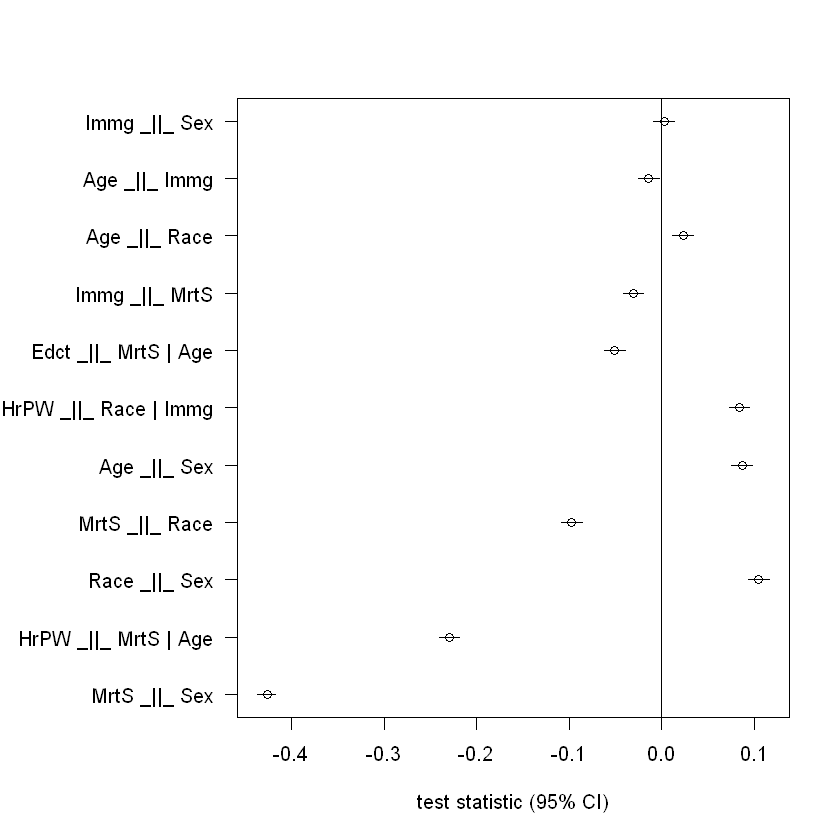
\includegraphics[scale = 0.5]{A2/Imagens/r2m2.png}
    \caption{Dados da Tabela \ref{r2m2} em uma representação visual.}
    \label{r2m2f}
\end{figure}

Agora, analisando os resultados da Figura \ref{r2m2f}, podemos ver que, com exceção da correlação entre estado civil e sexo, as variáveis que mais fogem do modelo proposto são a carga horária semanal com o estado civil, por meio da variável idade. Dessa forma, ao determinar uma relação entre tais variáveis deve-se ter um melhor ajuste do modelo.

\section{Conclusão}
\justify

Nesse trabalho pode-se ter uma ideia de como se utilizar Grafos Direcionados Acíclicos para a Inferência Causal por meio de um exemplo com um dataset sobre a renda populacional estadunidense. Pode-se ver que os DAGs modelam a independência entre as variáveis, apresentando o p-valor para a hipótese de independência, bem como um intervalo de confiança para a correlação das variáveis que, pelo modelo, foram julgadas independentes.

Quanto aos modelos, pôde-se perceber que o segundo modelo apresentado se sai um pouco melhor, fato dado pela inclusão de uma relação causal da variável ``Hours per Week'' com as variáveis ``Age'', ``Sex'' e ``Immigrant'', justamente o que pôde-se ver que estava defasado pela análise do primeiro modelo. Nota-se também uma grande correlação entre ``Sex'' e ``Marital Status'', a qual já foi explicada pela composição do dataset em si.

Por fim, pôde-se perceber que utilizar DAGs pode ser uma atitude poderosa para a modelagem de inúmeros fenômenos, especialmente quando quem está realizando a modelagem já possui algum conhecimento prévio sobre o dataset, bem como quando o fenômeno modelado pode ser bem explicado pelo modelador, seja em termos de complexidade ou de lógica na modelagem mesmo.

\newpage
\begin{thebibliography}{9}

\bibitem{dua2019} Dua, Dheeru and Graff, Casey. (2017). {UCI} Machine Learning Repository. \textit{University of California, Irvine, School of Information and Computer Sciences}. \url{http://archive.ics.uci.edu/ml}

\bibitem{ct} Ankan, A., Wortel, I. M. N., \& Textor, J. (2021). Testing graphical causal models using the R package ``dagitty''. \textit{Current Protocols, 1, e45}. doi: \url{https://doi.org/10.1002/cpz1.45}.

\bibitem{github} Michels, I. (2021). Statistical Modeling. \textit{Statistical Modeling}. \url{https://github.com/IgorMichels/Statistical_Modeling}

\bibitem{wiki} Directed Acyclic Graph. \textit{Wikipedia}. \url{https://en.wikipedia.org/wiki/Directed_acyclic_graph}.

\end{thebibliography}

\end{document}
